\chapter{Programming with Pluto}
\label{cap4}

In this chapter we present our solution to the issues introduced by the indoor context, its system architecture and, in the last section, how we achieved this result. We already said our goal is to complete user-defined missions, using nano-drones in an indoor context. We chose the Team Level approach, which we described in section ~\ref{teamlevel} to manage the missions assignment because, as we have shown in Section~\ref{teamlevelproblems}, the Team-Level approach is the most suitable approach for the kind of applications that can be developed with our framework.
The most important advantage of this approach is the reduced complexity given to the final user, while expressing the sensing tasks: there is no need to describe how the drones should execute them; these details are chosen by the Ground Control Station whose duty is to assign the right drone to the right task and check that each drone take its mission to the end with a successful status.


\section{System's architecture}
Pluto programming framework consists in two main components:
\begin{itemize}
\item Pluto Graphical Editor.
\item Pluto Main Application.
\end{itemize}
The former is used by the first actor of the Pluto life-cycle: a developer. The latter is used by a final user whose duty is to insert the sensing task and start their execution.
As you can see in figure \ref{fig:lifeCycle}, Pluto Graphical Editor lets the developer to creates a scenario based on the Team Level approach as we show in Section ~\ref{plutoGraphicalEditor}. After that, the Pluto Main Application is generated based on the diagram created in the previous step, so that the final user needs only to insert the sensing task and wait for their accomplishment.

\begin{figure}[htb]
  \centering
  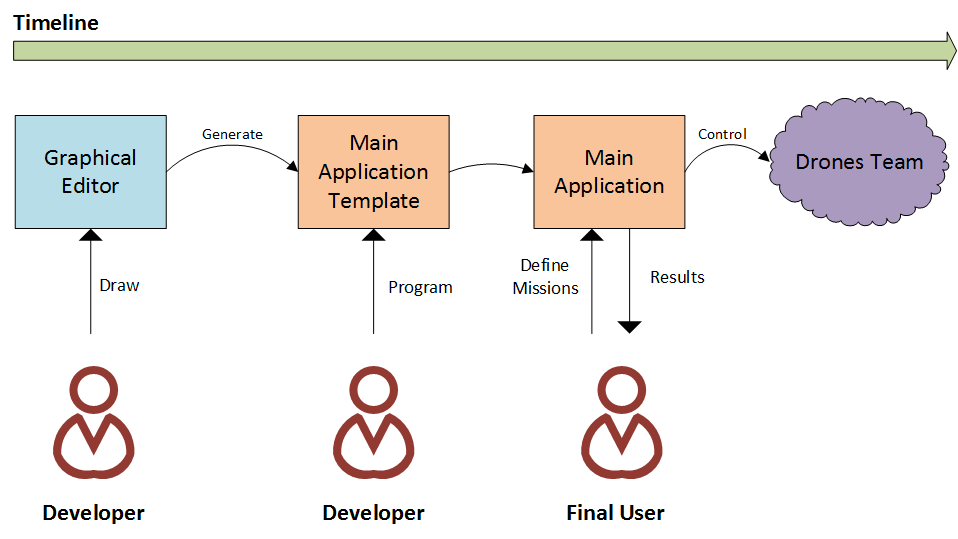
\includegraphics[width=\linewidth]{pictures/lifeCycle.png}
  \caption{A complete life cycle of the application}
  \label{fig:lifeCycle}
\end{figure}

\subsection{Pluto Graphical Editor}
\label{plutoGraphicalEditor}

We created a Graphical Editor in order to give freedom to the developer while designing the final app. The provided tools can be used to link together different kind of blocks, each one with a predefined and implemented logic.
When the Editor starts, it shows three main sections: the Palette that contains all the tools available to create a fully functional diagram; the Editor space, where the user can move, link, manage all the created entities; last but not least is the outline with a tree-view of the blocks created by the developer in the editor space.

\begin{figure}[htb]
  \centering
  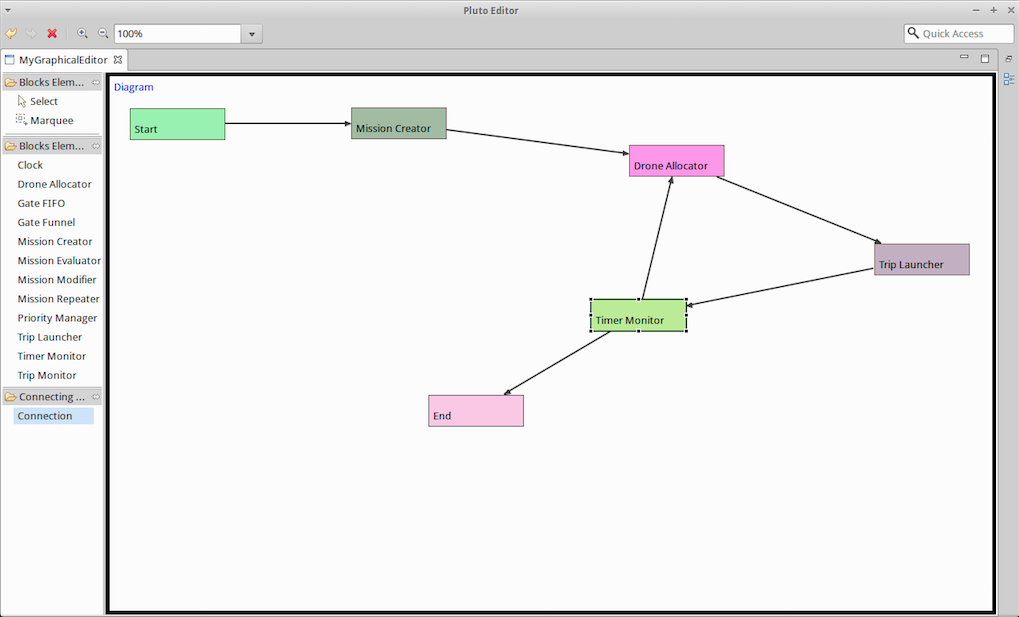
\includegraphics[width=\linewidth]{pictures/EditorScreen.png}
  \caption{Pluto Graphical Editor interface}
  \label{fig:GraphicalEditor}
\end{figure}

The developer can choose among several types of pre-created blocks, each one containing a certain logic, explained in (section~\ref{entities}). Creating a block in the editor space can be done simply with a drag and drop gesture or clicking on the desired entity and then clicking on the chosen location in the editor. Then the user can connect blocks each other using the Connection tool in the Palette section.
Apart from the standard functionality, such as Undo, Save, and Load, the Context Menu provides a command to generate a source-code of the Main Application based on the designed diagram. Toolbar provides Undo/Redo, Delete, and Magnify commands.
To understand better Pluto Graphical Editor, it's worth to spend a word on the meaning of creating a diagram: each block in the Diagram is black box which is intended to manage a Mission entity. It takes a Mission as an input, works with it and sends it out as an output. The connections among blocks represents the path that the Mission entity will follow after going out from a block. Each block could have multiple outgoing and incoming connections.
In the end, on the editor, the developer will have a set of blocks linked together with a set of connections. This drawing can be interpreted as the behavior of the Main Application in managing the missions. For example we designed a sketch of a possible diagram, as shown in figure ~\ref{fig:GraphicalEditor}. This design is very simple and could be a first skeleton for a more complex application, by simply adding new blocks.
Besides of simplicity, our editor is very flexible as well, since it provides a Mission Modifier block whose implementation logic can be written directly in the Editor right-clicking on the block and choosing the option "Write Custom Code". This will be explained better in section~\ref{entities}

\subsection{Pluto Main Application}
\label{plutoMainApp}

The Pluto Main Application is the final application that act as a Ground Control Station, managing all the drones and the missions. In this section we explain how it works.
Everything starts in the Mission Page where the user can define the tasks that will be carried out by the drones. After clicking to the "Add Mission" button the user is asked to set a name for the mission.

\begin{figure}[htb]
  \centering
  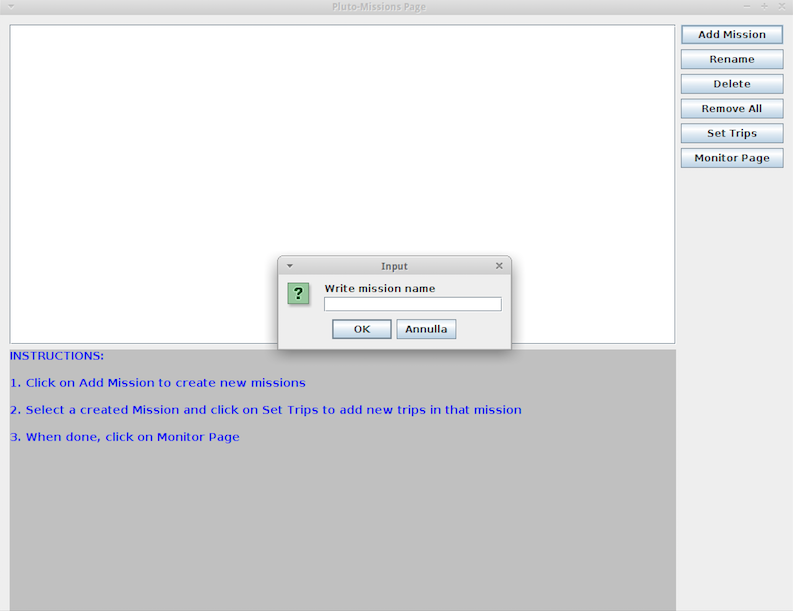
\includegraphics[width=\linewidth]{pictures/MissionPage.png}
  \caption{Mission Page interface}
  \label{fig:MissionPage}
\end{figure}

Then, the user is asked to decide if the mission must be repeated. If he click "Yes", that mission will continue to execute cyclically until the user decide to stop it, through the Stop button of the Monitor Page.

\begin{figure}[htb]
  \centering
  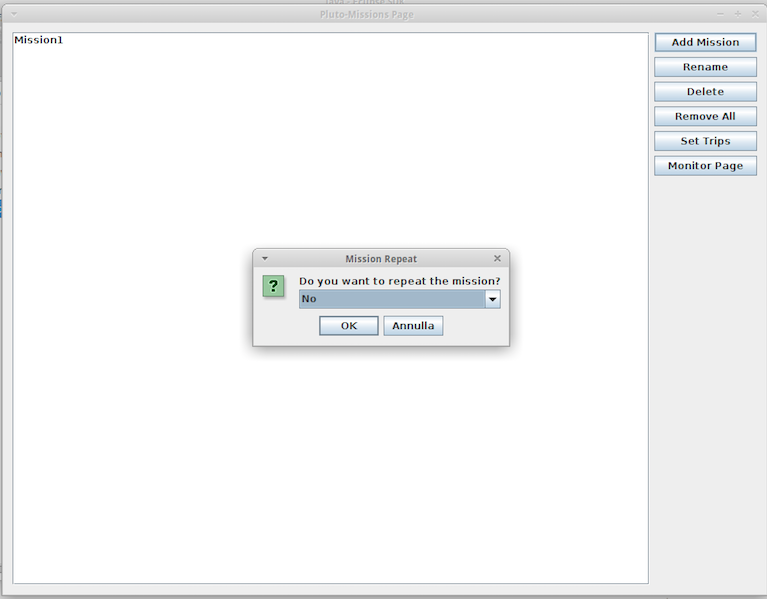
\includegraphics[width=\linewidth]{pictures/missionRepeat.png}
  \caption{Mission Repeatable pop up}
  \label{fig:missionRepeat}
\end{figure}

After that a Mission entity is created, but by now it doesn't contain any information about what has to be done. To add this information the user has to double-click on the mission in the main list or click on the "Set Trips" button. A new window will appear, as shown in figure  ~\ref{fig:TripsPage}, and the user can add Trips entity to the related Mission. A Trip is nothing but a movement from point A to point B inside our indoor context. Trips are the basic entities that constitute a single Mission. The single Trip contains information about the Action to execute once point B is reached. Furthermore the Trip has a reference of the drone assigned to it, but we will talk about this in section ~\ref{entities}.

\begin{figure}[htb]
  \centering
  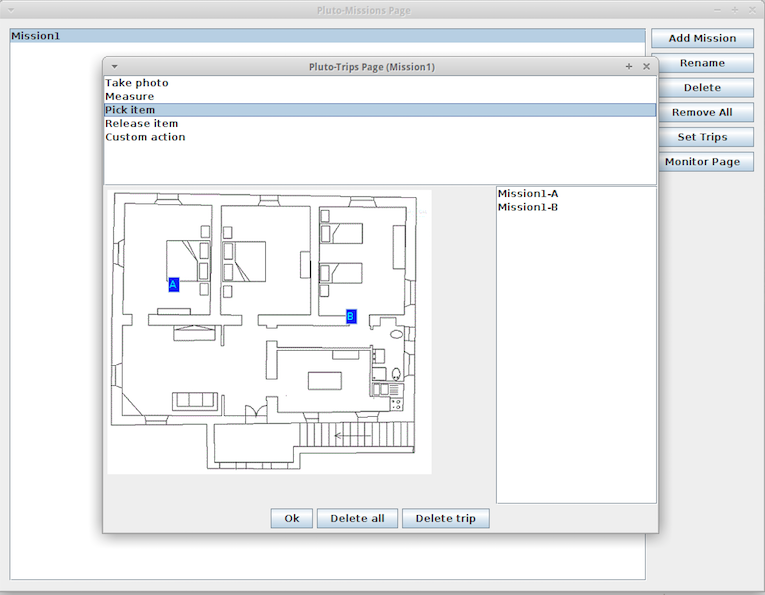
\includegraphics[width=\linewidth]{pictures/TripsPage.png}
  \caption{Trips Page interface}
  \label{fig:TripsPage}
\end{figure}

So after all the Trips are added to a single Mission the user can create more Mission or pass to the Monitor Page with the corresponding button.
The Monitor Page, shown in figure ~\ref{fig:MonitorPage}, is the window where the user can obtain information about the running missions, at run-time. On the top, there is a table where each row is assigned to a Mission, each column will display the information about the current Trip that is executing and the Drone that has been assigned to that Trip.
Below the table there is a console where log messages are printed during the execution of each missions. In this way the user can obtain run-time information about the status of the entire system. 
Of course the Start button will start the execution of the created missions, while the Stop button will prompt the user to a behaviour choice: "RTL" or "Land". The first will make all drones to return to the home location instantly, while the second option will make all drones to land in their current locations. After the Stop command, the missions status will be preserved and could be continued in the future.

\begin{figure}[htb]
  \centering
  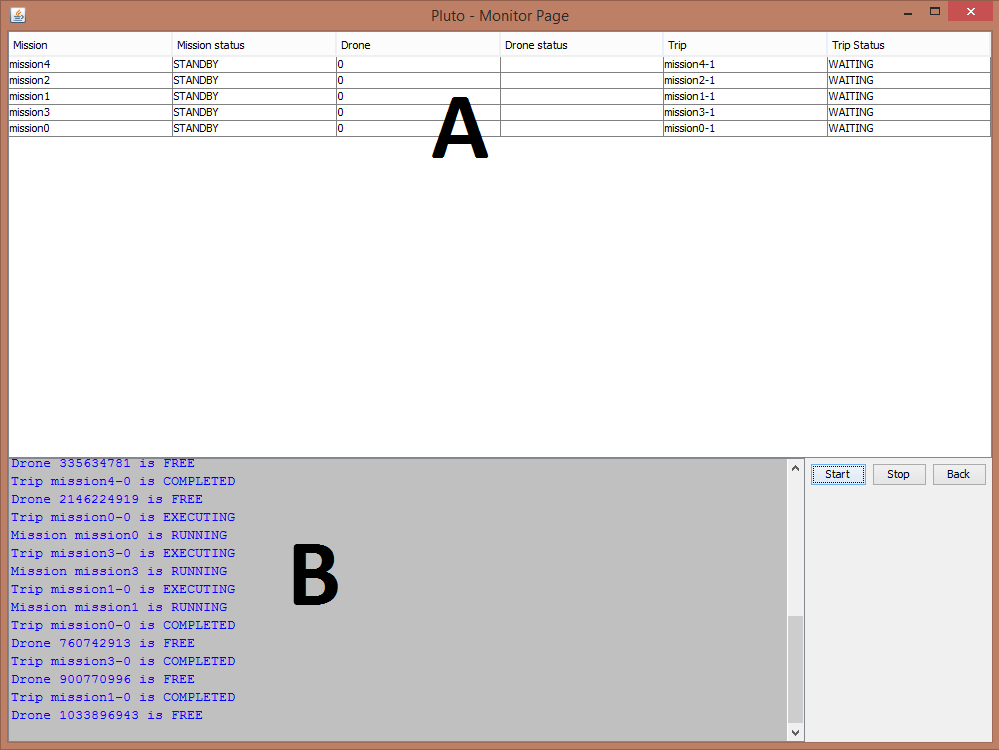
\includegraphics[width=\linewidth]{pictures/MonitorPage.png}
  \caption{Monitor Page interface}
  \label{fig:MonitorPage}
\end{figure}

\newpage

\section{Dataflow model}\label{dataFlow}

In this section we present the Dataflow model in a complete and sound way.
First, we describe a general view of the model in Section ~\ref{descriprionOfModel}. Then, in Section ~\ref{modelRepresentation} we focus on the details of the each component of the model.


\subsection{Description of the model}
\label{descriprionOfModel}

Each diagram created with the Pluto Graphical Editor is made of many functional blocks, each one is implemented with a particular logic; the user can select the blocks needed for his particular application and connect them through simple links, as explained in section~\ref{plutoGraphicalEditor}.
In the figure~\ref{fig:BlocksDiagram}, an example application is showed, which contains some of the implemented blocks.
Again, the user is not forced to insert all the blocks, he can choose only the blocks needed for his particular application.
If you compare this figure with figure~\ref{fig:GraphicalEditor}, you can see that this one is based on the the same drawing but with additional features provided by new blocks.
\\

\begin{figure}[htb]
  \centering
  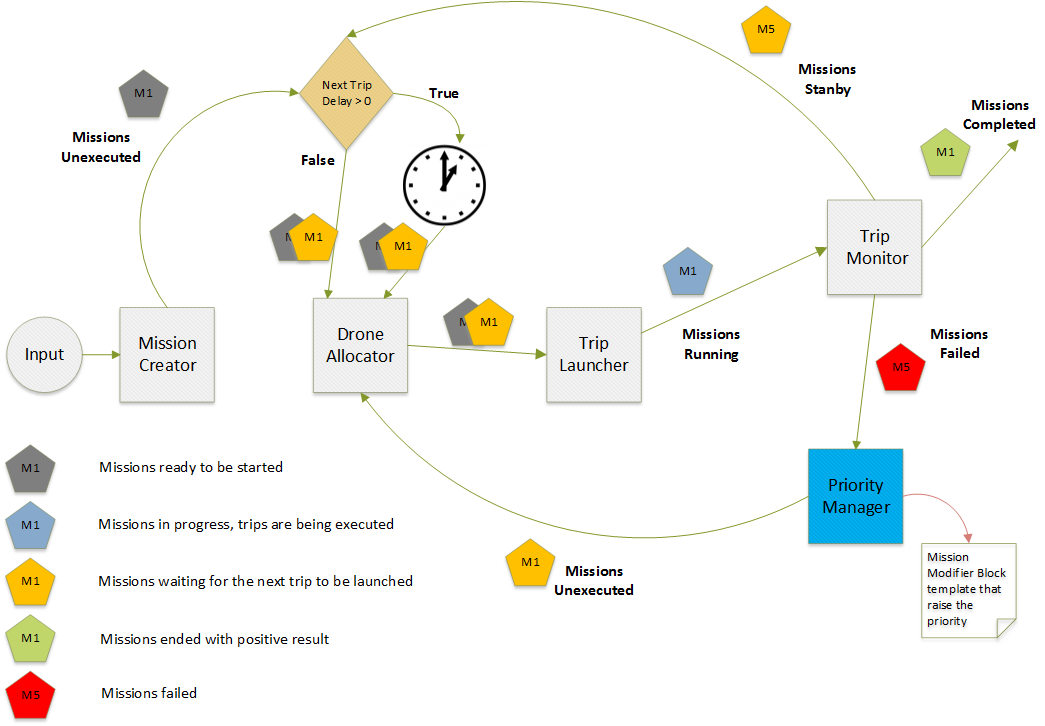
\includegraphics[width=\linewidth]{pictures/BlocksDiagram.png}
  \caption{An example Pluto application}
  \label{fig:BlocksDiagram}
\end{figure}


\newpage
\subsection{Model representation}
\label{modelRepresentation}
In this section we show the fundamental entities of our model, in order to better understand the functioning of the blocks. Then, all the blocks of figure ~\ref{fig:BlocksDiagram} are described in details, explaining what tasks they perform and showing a pseudo-code representation for each of them.

\subsubsection {Entities}
\label{entities}

Basically, through the interface presented in section~\ref{plutoMainApp}, the user specifies a list of Missions that the system must perform; each Mission contains a list of Trips; a Trip is a path between a start location and a target location; the Trip is performed by a Drone which carries out an Action, for example it can bring an Item to a person, or take a photo or measure temperature at a particular location.

So we identified the following entities:

\begin{itemize}
\itemsep2pt
\item{
Mission
}
\item{
Trip
}
\item{
Drone
}
\item{
Action
}
\item{
Item
}
\end{itemize}

As shown in figure~\ref{fig:EntityRelationship}, the Mission entity, in addition to the set of Trips, has another important attribute that is the Status: it describes how the Mission is being executing.
\\
The Trip entity has a Status attribute too and furthermore it contains the Drone and the Action entities. Then of course the coordinates of the source and the target locations.
\\
The Drones are described by an unique ID and by a shape category which tell the system what kind of items can be hold by the drone.
\\
Regarding the Action entity, a very important feature is the \textit{Custom Action}: it allows the programmer to implement a new action that the drones can perform.
It obviously depend on the particular application, but for example a programmer can add the Pollinate action needed for the Alfalfa application\cite{alfalfa}, which will be described in section \ref{alfalfa}.
\\
The code implementation of these classes can be found in section~\ref{oomodel}.

\newpage

\begin{figure}[htb]
  \centering
  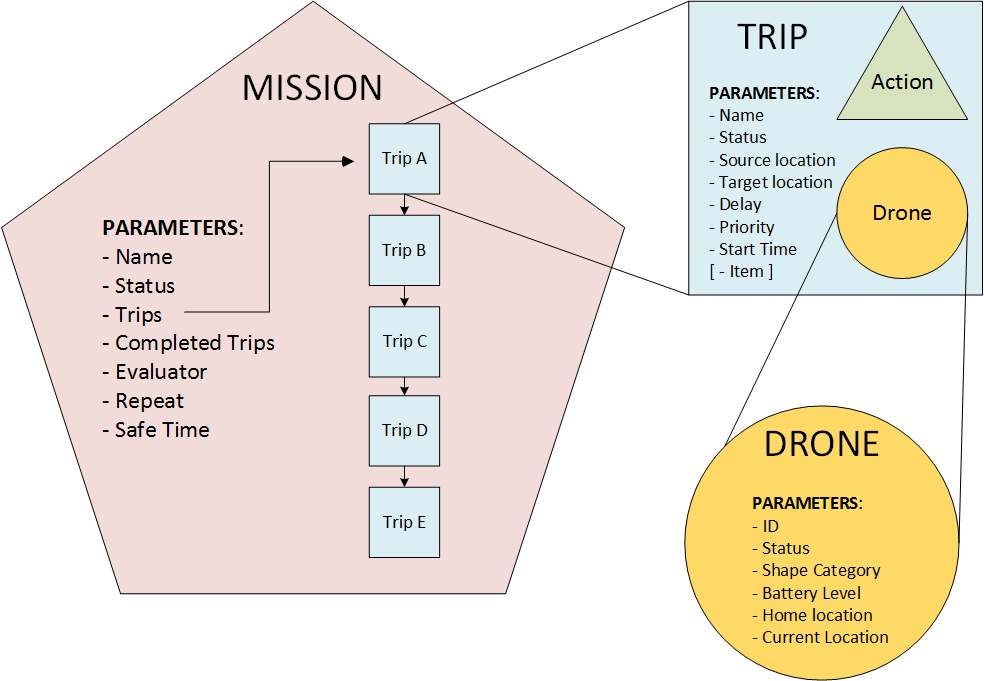
\includegraphics[width=\linewidth]
  {pictures/EntityRelationship.png}
  \caption{Relationship among model entities}
  \label{fig:EntityRelationship}
\end{figure}


\subsubsection {Description of the blocks}\label{blocks}

Here we provide a detailed description of each functional block available in the Pluto Graphical Editor:
\\

\underline{Mission Creator block}
\\

input: a list of Trips

output: a Mission object
\\

The Mission Creator block receives as input the trips that the user wants to be performed by the drones, then it creates a Mission including all these trips and returns that Mission object.
This block is the starting point of each Pluto-developed application.
\\



\underline{Clock block}
\\

input: a Mission object

output: a Mission object
\\

The Clock block checks the delay attribute of each Trip of a Mission: if it's not equal to zero, it makes the Trip wait for the amount of time set by the user in the Mission creation step, and finally returns the Mission Object.
If the programmer puts the Clock block in the graph of the application, the Pluto Main application shown in section \ref{plutoMainApp} will show an extra widow.
On the Trips Page,after the final user drags and drops on the map the action to perform and the Priority panel is shown, the user will be asked to set a delay for the Trip.
This block has to be put between the Mission Creator and the Drone Allocator blocks.
\\

\underline{Drone Allocator block}
\\

input: a Mission object

output: a Mission object
\\

The DroneAllocator block chooses the appropriate Drone to be assigned to each Trip, basing on the availability of the drones and their capability to perform the desired action.
The output of the DroneAllocator is always sent to the TripLauncher, while its input can arrive from a variety of blocks, depending on the features of the considered application.
\\

\underline{Trip Launcher block}
\\

input: a Mission object

output: a Mission object
\\
The TripLauncher block takes the next Trip to be performed from the Mission object, and launches it.
The assigned drone will fly to the target location and execute the defined Action.
This block receives the input Mission from the DroneAllocator block, ans sends its output to the TripMonitor.
If the application contains the TimerMonitor block, the TripLauncher's output will be also sent to it.
\\

\underline{Trip Monitor block}
\\

input: a Mission object

output: a Mission object
\\

The TripMonitor block checks the status of the Trip that is running in that moment.
It changes the status of the Trip and of the Mission in the appropriate way, depending on whether the Trip is failed or complete.
This block receives the input Mission from the TripLauncher, and its output can be sent to the GateFIFO, the MissionEvaluator or the DroneAllocator blocks, depending on the features of the particular application.
\\



\underline{Mission Repeater block}
\\

input: a Mission object

output: a Mission object
\\

The MissionRepeater block verifies if the \textit{repeat} attribute of the input Mission is set to true.
If so, it set the Mission status to STANDBY and the status of all the Trips of that mission to WAITING and inserts again them in the List of Trips to be executed.
This block is put between the MissionEvaluator and the DroneAllocator.
\\

\underline{Gate FIFO block}
\\

input: a Mission object

output: a Mission object
\\

The GateFIFO block is used when two or more blocks works in parallel, and only one instance of the executing Mission must propagate.
Among the multiple input connections of the GateFIFO block, it propagates only the one that completed its task for first.
That's why the FIFO acronym is used, since the first Mission instance that arrive is the only one that propagates in the graph.
This block receives the input Mission from one of the blocks connected to it and can send its output to the MissionEvaluator, MissionRepeater or DroneAllocator blocks, depending on the particular application.
\\

\underline{Mission Evaluator block}
\\

input: a Mission object

output: a Mission object
\\

The MissionEvaluator block can read and write data carried by the drones, and basing on them can perform various actions specific for the application developed.
It receives the input Mission from the GateFIFO or TripMonitor blocks and can send the output to the DroneAllocator or MissionRepeater blocks, depending on the particular application.
\\

\underline{Mission Modifier block}\label{mm}
\\

input: a Mission object

output: a Mission object
\\

The MissionModifier block allows the programmer to create new custom blocks.
As shown in figure~\ref{fig:missionmodifier}, in the editor, he can inserts his custom code in this block using the appropriate option in the context menu.
This block can be put in every point of the Pluto Editor graph, depending on the particular feature it implements.
\\

\begin{figure}[H]
\centering
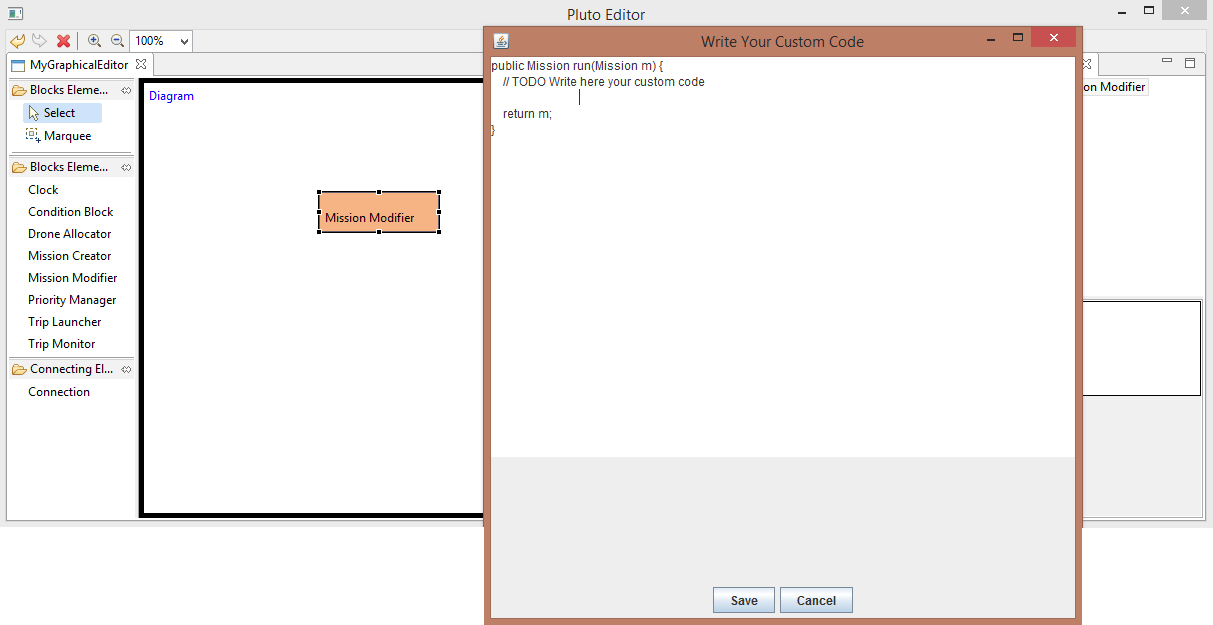
\includegraphics[width=\linewidth]
{pictures/MissionModifier.png}
  \caption{The MissionModifier block}
  \label{fig:missionmodifier}
\end{figure}

\underline{PriorityManager block}
\\

input: a Mission object

output: a Mission object
\\

The Priority Manager block raise the priority of the first Trip of the Mission passed in input.
This block can be considered as a particular case of Missio nModifier. 
This block can receive the input from the Gate Fifo or Trip Monitor blocks, and sends the output to the Drone Allocator.
\\

\underline{Timer Monitor block}
\\

input: a Mission object

output: a Mission object
\\

The TimerMonitor block takes the input mission and waits for the completion of the current running Trip. If the Trip doesn't end before the fail-safe time, it will set the status of the Trip and of the Mission both to FAILED, then it will put the mission as output.
This block can be considered as a particular case of MissionModifier.
It's always put between the TripLauncher and the GateFIFO blocks.
\\

\underline{Gate Funnel block}
\\

input: a Mission object

output: a Mission object
\\

Similar use of the GateFIFO, but this gate will wait for all the Mission instances that are being managed before this block. So if before this gate, there are 4 blocks in parallel that are managing their Mission instance, the propagation of the Mission after this gate will be activated only when all the 4 instances will arrive.
\\

\underline{Start block}
\\
State the beginning of the diagram
\\

\underline{End block}
\\
State the end of the diagram, where the completed missions will go into.
\\

\section{Aiming to the final model}

In this section we describe our previously developed solutions, which we refined many times in order to obtain the final working version of the Pluto programming framework; this is done by using a top-down approach, starting from the final implementation to the very first one.

\subsection{Solution without Trip entity}

In the version precedent to the final solution, presented in section~\ref{dataFlow}, we did not have a concept of Trip, and Mission was the main concept the whole model was based on. The following diagrams shows this in the particular case of the Timer feature, which contains also a "Switch source-target" block. Later, this block was included in the logic of the Trip.

\begin{figure}[htb]
  \centering
  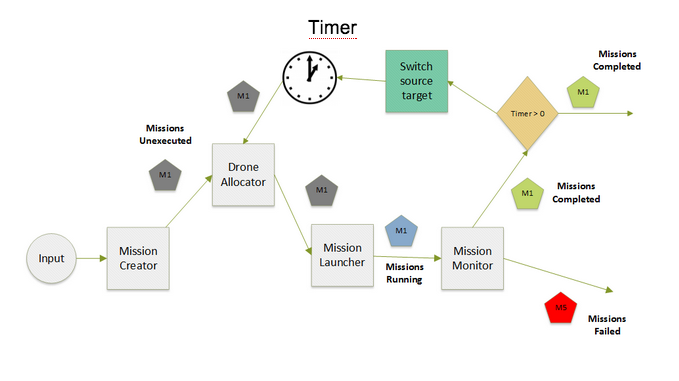
\includegraphics[width=\linewidth]{pictures/NoTrip.png}
  \caption{Solution without the Trip concept}
  \label{fig:noTrip}
\end{figure}

After analysing the model, we realized that we needed the concept of Trip, because the final user must have control on the single Trip of a drone, in order to decide which action the drone must perform, and to have an opportunity to control the Trip such as delay, stop, or delete, without deleting or stop the whole Mission. With this precedent solution it is not possible, because having only the entire  Mission to manage, the user can no control the single Trip, and if he/she wants to delete only a part of the Mission he cannot do so, and he/she is forced to delete and build again the whole Mission.

\subsection{Solution without the DroneAllocator}


This solution instead of the DroneAllocator block, used the "Drone Updater" one. This block managed the assignment of the Drone to a Mission, only in special conditions. This means that, generally, there were no need of this block unless the developer put some special block such as the old TimerMonitor or the old DelayMonitor.
In this solution, the MissionCreator managed the assignment of a Drone to the Mission. This is the reason why we didn't need the DroneUpdater in normal conditions.
As said, there were also the "Delay Monitor" and "Timer Monitor" blocks, instead of the Clock block.
These blocks managed the delayed missions(fig.~\ref{fig:delayMonitor}) and the missions with an associated timer(fig.~\ref{fig:noClock}), respectively.
There wasn't the MissionModifier block, but only the "Priority Manager" one, so the programmer couldn't insert blocks(fig.~\ref{fig:noMM}) with custom code.

\begin{figure}[htb]
  \centering
  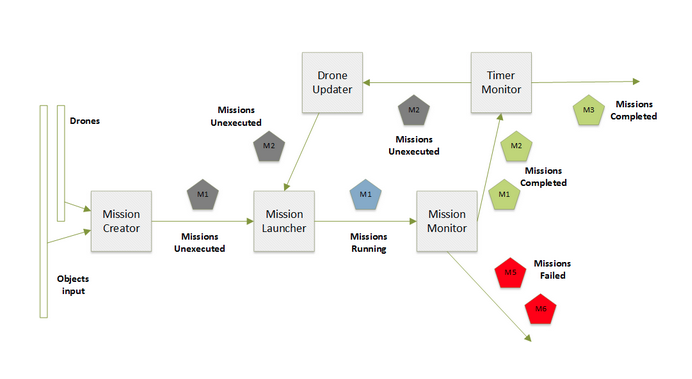
\includegraphics[width=\linewidth]{pictures/NoClock.png}
  \caption{Solution with the TimerMonitor}
  \label{fig:noClock}
\end{figure}


\begin{figure}[H]
  \centering
  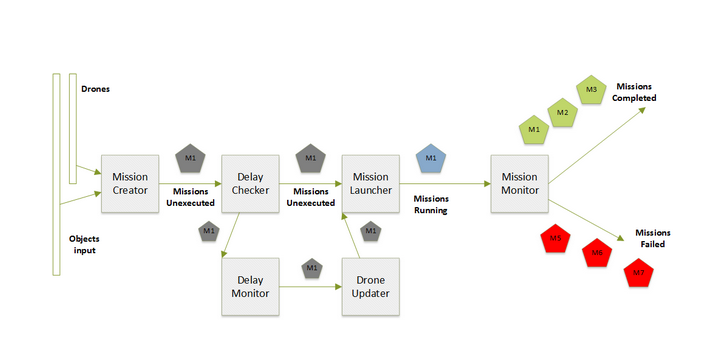
\includegraphics[width=\linewidth]{pictures/DelayMonitor.png}
  \caption{Solution with the DelayMonitor}
  \label{fig:delayMonitor}
\end{figure}

\begin{figure}[htb]
  \centering
  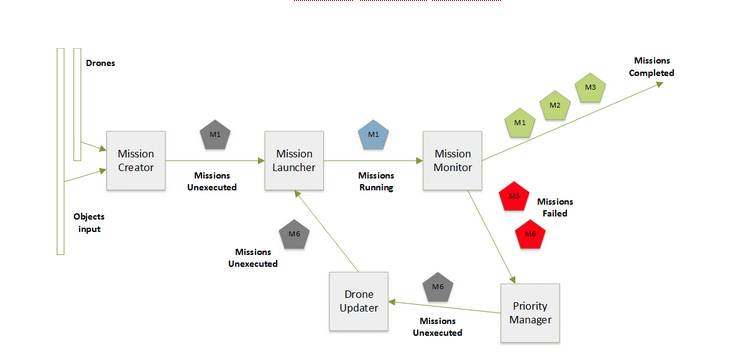
\includegraphics[width=\linewidth]{pictures/NoMM.png}
  \caption{Solution without the MissionModifier block}
  \label{fig:noMM}
\end{figure}

Actually we decided to put the DroneAllocator block because weneed to separate the creation of a Mission Object from the assignment of a Drone to it; in this way we could also remove the DroneUpdater block, because now we have an apposite block which manage only the assignment of Drones, so there is no more need to distinguish between the normal assignment and the special assignment(in the case of delayed trip).
Also the DelayMonitor and TimerMonitor blocks were useless, because there is no need to distinguish between a delay and a timer, so a single Clock block can manage these cases both.
In this solution only the PriorityManager block existed, but we decided to create a MissionModifier block in which the user can put his own code he needs for a particular application, so the PriorityManger block can be seen as a particular case of the MissionModifier one.